%%%%%%%%%%%%%%%%%%%%%%%%%%%%%%%%%%%%%%%%%
% Beamer Presentation
% LaTeX Template
% Version 1.0 (10/11/12)
%
% This template has been downloaded from:
% http://www.LaTeXTemplates.com
%
% License:
% CC BY-NC-SA 3.0 (http://creativecommons.org/licenses/by-nc-sa/3.0/)
%
%%%%%%%%%%%%%%%%%%%%%%%%%%%%%%%%%%%%%%%%%

%----------------------------------------------------------------------------------------
%	PACKAGES AND THEMES
%----------------------------------------------------------------------------------------

\documentclass{beamer}

\mode<presentation> {

% The Beamer class comes with a number of default slide themes
% which change the colors and layouts of slides. Below this is a list
% of all the themes, uncomment each in turn to see what they look like.

%\usetheme{default}
%\usetheme{AnnArbor}
%\usetheme{Antibes}
%\usetheme{Bergen}
%\usetheme{Berkeley}
%\usetheme{Berlin}
%\usetheme{Boadilla}
%\usetheme{CambridgeUS}
%\usetheme{Copenhagen}
%\usetheme{Darmstadt}
%\usetheme{Dresden}
%\usetheme{Frankfurt}
%\usetheme{Goettingen}
%\usetheme{Hannover}
%\usetheme{Ilmenau}
%\usetheme{JuanLesPins}
%\usetheme{Luebeck}
%\usetheme{Madrid}
\usetheme{Malmoe}
%\usetheme{Marburg}
%\usetheme{Montpellier}
%\usetheme{PaloAlto}
%\usetheme{Pittsburgh}
%\usetheme{Rochester}
%\usetheme{Singapore}
%\usetheme{Szeged}
%\usetheme{Warsaw}

% As well as themes, the Beamer class has a number of color themes
% for any slide theme. Uncomment each of these in turn to see how it
% changes the colors of your current slide theme.

%\usecolortheme{albatross}
%\usecolortheme{beaver}
%\usecolortheme{beetle}
%\usecolortheme{crane}
%\usecolortheme{dolphin}
%\usecolortheme{dove}
%\usecolortheme{fly}
%\usecolortheme{lily}
%\usecolortheme{orchid}
%\usecolortheme{rose}
%\usecolortheme{seagull}
%\usecolortheme{seahorse}
%\usecolortheme{whale}
%\usecolortheme{wolverine}

%\setbeamertemplate{footline} % To remove the footer line in all slides uncomment this line
%\setbeamertemplate{footline}[page number] % To replace the footer line in all slides with a simple slide count uncomment this line

%\setbeamertemplate{navigation symbols}{} % To remove the navigation symbols from the bottom of all slides uncomment this line
}

\usepackage{graphicx} % Allows including images
\usepackage{booktabs} % Allows the use of \toprule, \midrule and \bottomrule in tables

%----------------------------------------------------------------------------------------
%	TITLE PAGE
%----------------------------------------------------------------------------------------

\title[Global Illumination]{Screen-Space Global Illumination on Deep G-Buffers} % The short title appears at the bottom of every slide, the full title is only on the title page

\author{Jonas H. Nielsen} % Your name
\institute[DTU Compute] % Your institution as it will appear on the bottom of every slide, may be shorthand to save space

\begin{document}

\begin{frame}
\titlepage % Print the title page as the first slide
\end{frame}

\begin{frame}
\frametitle{Overview} % Table of contents slide, comment this block out to remove it
\tableofcontents % Throughout your presentation, if you choose to use \section{} and \subsection{} commands, these will automatically be printed on this slide as an overview of your presentation
\end{frame}

%----------------------------------------------------------------------------------------
%	PRESENTATION SLIDES
%----------------------------------------------------------------------------------------

%------------------------------------------------
\section{Deferred Rendering} 

\begin{frame}
\frametitle{Deferred Rendering Overview}
\begin{itemize}
\item Draw geometric information to off-screen textures.
\item Use off-screen textures to do shading at later stage.
\item Abstracts shading calculations from geometric complexity.
\end{itemize}

\begin{center}
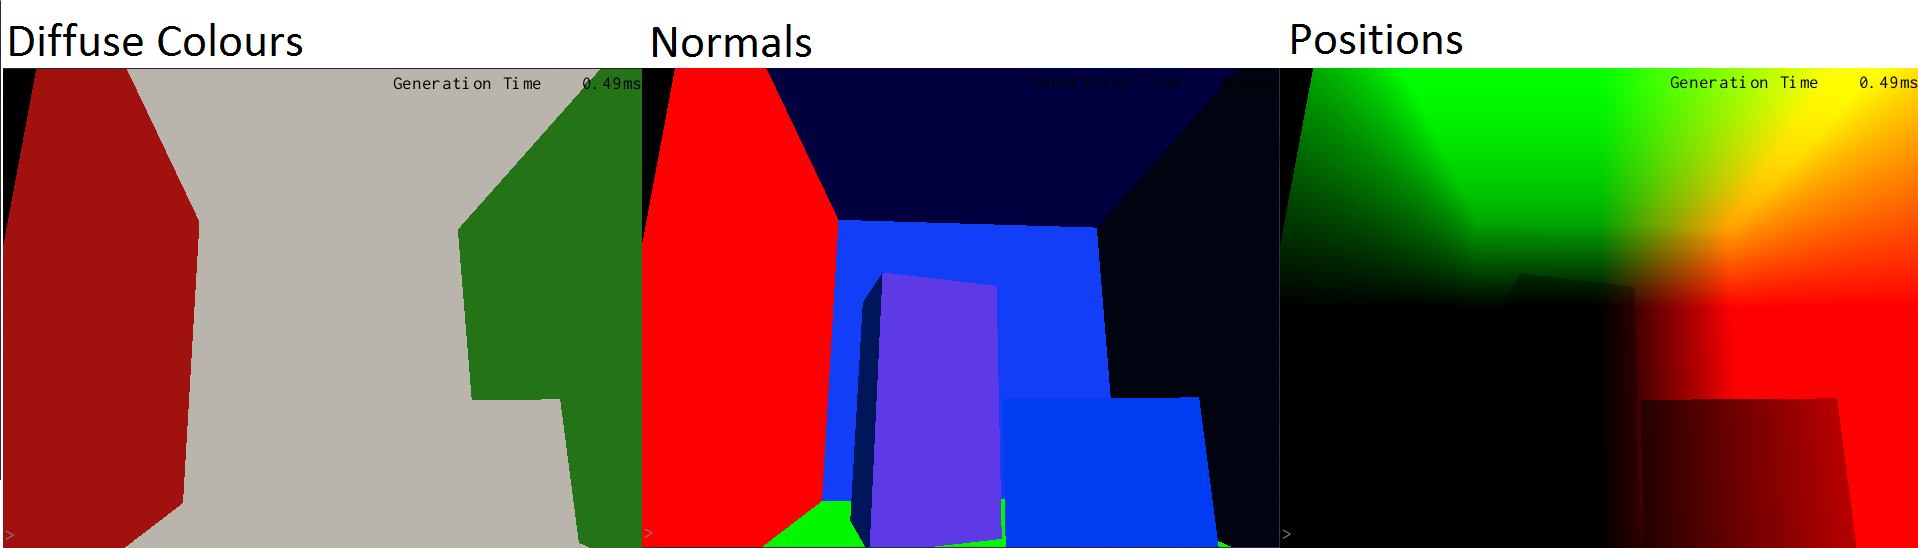
\includegraphics[scale=0.2]{img/def-rend/all}
\end{center}
\end{frame}

%------------------------------------------------

\subsection{Deep G-buffer} 

\begin{frame}
\frametitle{Deep G-buffer}
\begin{itemize}
\item Store multiple layers of geometry in off-screen targets.
\item Determine lower layer contents by contents of upper layers.
\item Use geometry shader to do in a single pass
\item Use previous frame's depth buffer to predict contents.
\end{itemize}

\begin{center}
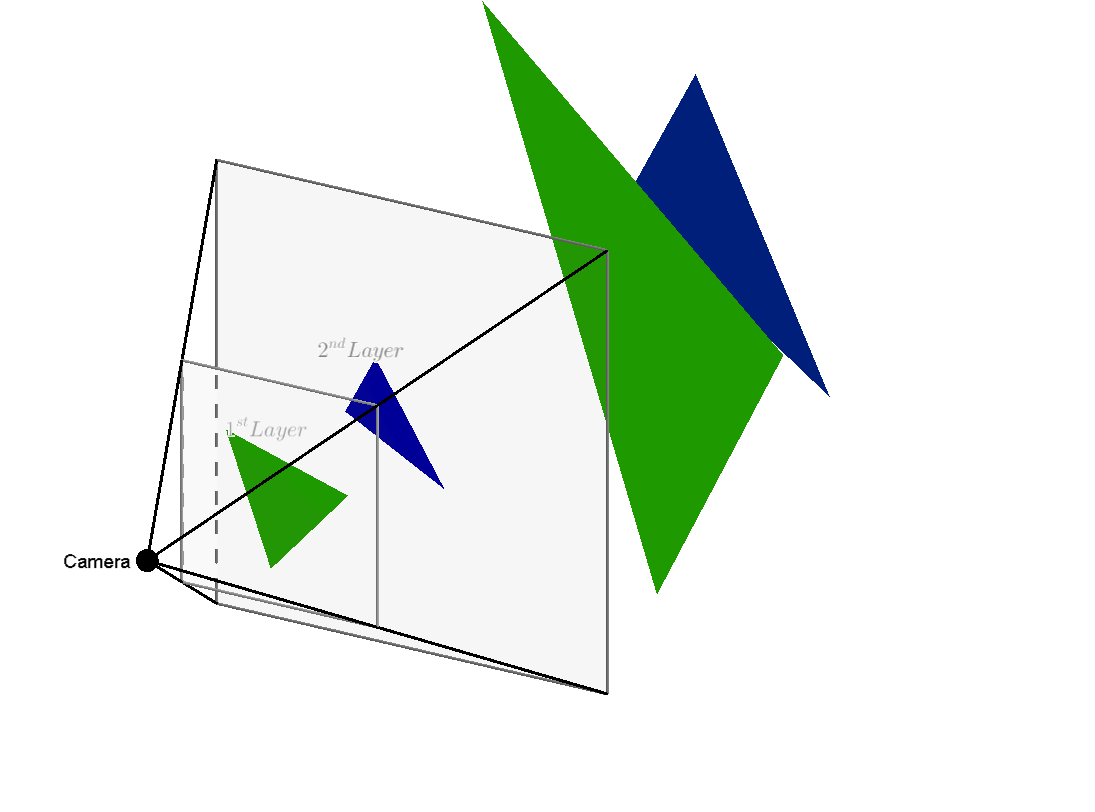
\includegraphics[scale=0.8]{img/2-layer}
\end{center}
\end{frame}

%----------------------------------------------------------------------------------------

\subsection{Scene Reconstruction}

\begin{frame}
\frametitle{Scene Reconstruction}
\begin{itemize}
\item Reconstruct geometric information.
\item Allows to buffer less data, by reconstruction.
\item Use inverse projection matrix to get view-space coords.
\item Less VRAM writes and reads vs reconstruction cost.
\end{itemize}
\end{frame}

%----------------------------------------------------------------------------------------

\section{Omni-directional Shadowmapping}

\begin{frame}
\frametitle{Cube Shadow Mapping}
\begin{itemize}
\item Render vertex-depth unto a cube map.
\item Use vertex view-length as depth.
\item Center view-matrices around light position.
\item Adjust up-, and at-vectors according to sides of cube.
\item Rasterise in single pass with geometry shader.
\end{itemize}
\end{frame}

\begin{frame}
\frametitle{Shadow Results}
\begin{center}
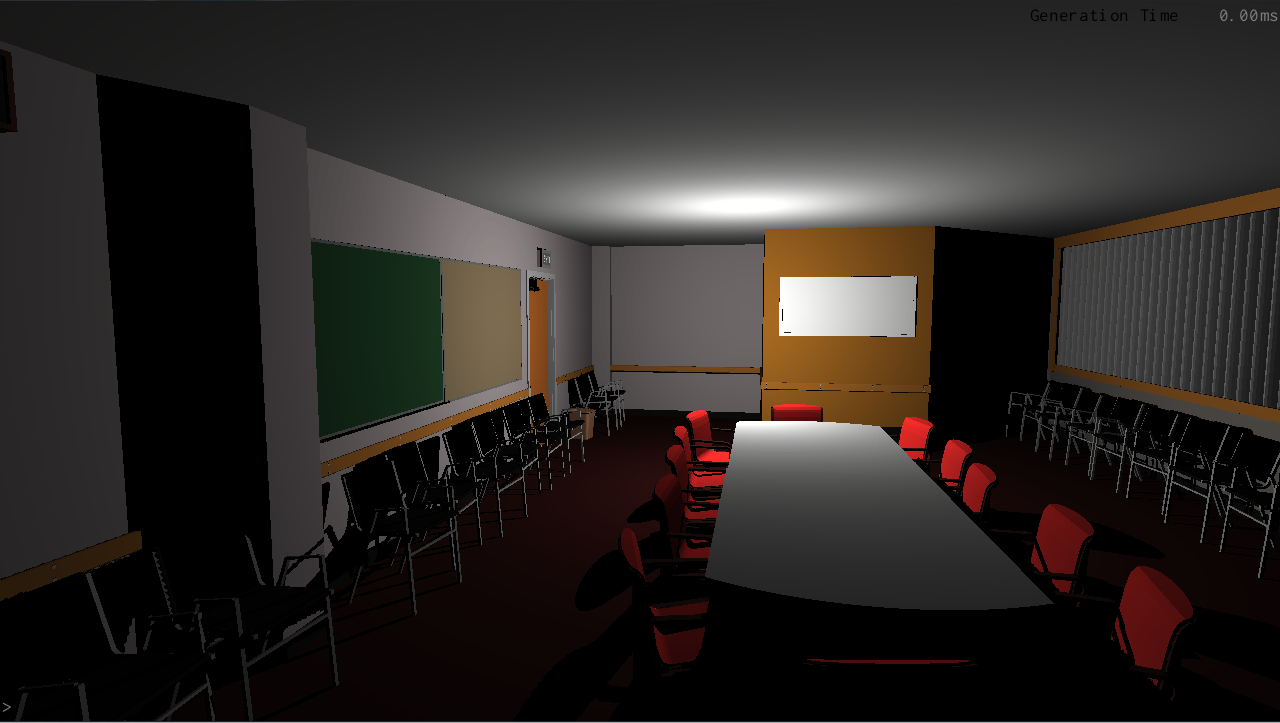
\includegraphics[scale=0.3]{shadow}
\end{center}
\end{frame}

%----------------------------------------------------------------------------------------

\section{Filters}

\begin{frame}
\frametitle{Sampling Strategy}
\begin{itemize}
\item Sample in screen-space along a spiral curve.
\item Use parameters to impact form of curve.
\end{itemize}
$$\sigma = t + \frac{\psi}{\tau} $$
$$\theta = 2\pi\sigma\tau + \phi $$
$$\overline{u} = \begin{pmatrix}\cos(\theta) \\ \sin(\theta) \end{pmatrix} $$
$$h = R \sigma $$
$$\mathbf{v} = h \overline{u}$$
$$0 < t < 1, 0 < \phi < 2\pi, 0 < \psi < 1$$
\end{frame}


\subsection{Radiosity}

\begin{frame}
\frametitle{Radiosity Equation}
\begin{itemize}
\item Rendering equation for radiosity:
$$B(\mathbf{X}) = \int_\Omega \frac{\rho_d}{\pi} B(\mathbf{Y}) \cos(\theta) V() d\omega_i$$
\item Monte-Carlo Approximation:
$$B(\mathbf{X}) = \sum_{i=0}^{n} \frac{\rho_d}{\pi} B(\mathbf{Y}(\omega_i)) \cos(\theta) V() \Delta \omega_i$$
\end{itemize}
\end{frame}

\begin{frame}
\frametitle{Solving $\Delta \omega_i$}
\begin{itemize}
\item Assume all samples represent equal solid angles:
$$B(\mathbf{X}) = \frac{2\pi}{n} \frac{\rho_d}{\pi} \sum_{i=0}^{n} B(\mathbf{Y}[\omega_i]) \cos(\theta)V()$$
\item Weight based on surface differential:
$$\Delta \omega_i = 2\pi \frac{\frac{\cos(\phi)}{\pi r^2}}{M}$$
$$M = \sum_{i = 0}^{n}\frac{\cos(\phi)}{\pi r^2}$$
$$B(\mathbf{X}) = \frac{2\pi}{M} \frac{\rho_d}{\pi} \sum_{i=0}^{n} B(\mathbf{Y}[\omega_i]) \cos(\theta)V()\frac{\cos(\phi)}{r^2}$$
\end{itemize}
\end{frame}

\begin{frame}
\frametitle{Simple method result}
\begin{center}
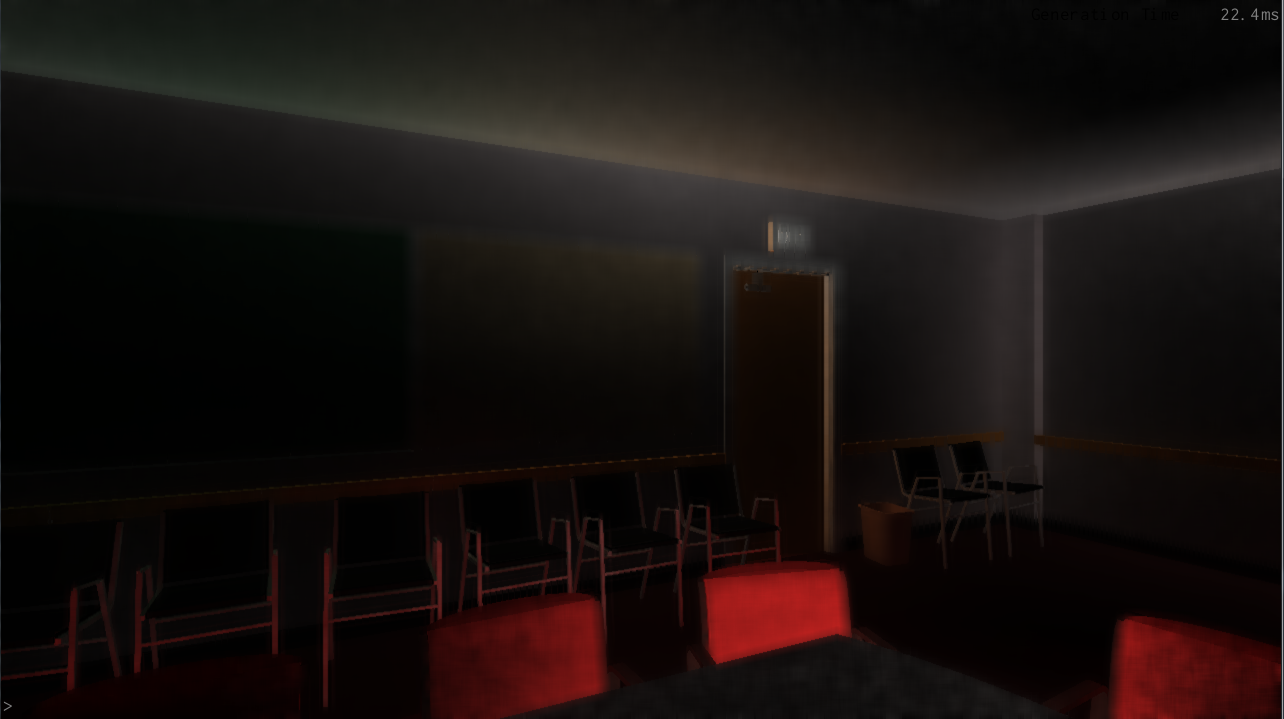
\includegraphics[scale=0.3]{img/w-edge-rad}
\end{center}
\end{frame}

\begin{frame}
\frametitle{Alternate Method Result}
\begin{center}
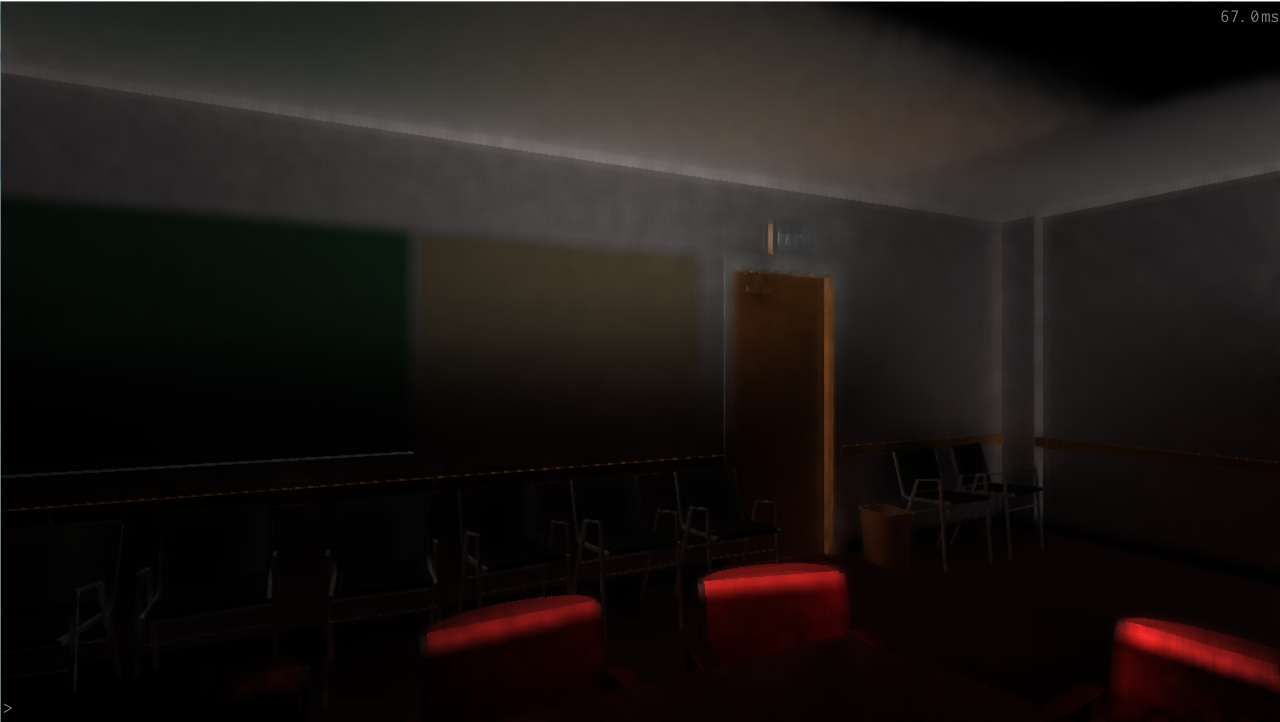
\includegraphics[scale=0.3]{img/newdomega}
\end{center}
\end{frame}

\begin{frame}
\frametitle{Timings for different $d\omega$s}
\begin{center}
\begin{tabular}{|r|r|r|}
\hline
\multicolumn{1}{|l|}{} & \multicolumn{1}{c|}{$2\pi \frac{\cos(\phi)}{r^2 M}$} & \multicolumn{1}{c|}{$\frac{2\pi}{M}$} \\ \hline
\multicolumn{1}{|l|}{\textit{Samples}} & \multicolumn{1}{l|}{\textit{Time (ms)}} & \multicolumn{1}{l|}{\textit{Time (ms)}} \\ \hline
10 & 19,8 & 13,3 \\ \hline
15 & 27,6 & 17,9 \\ \hline
20 & 35,6 & 22,5 \\ \hline
25 & 43,6 & 27,1 \\ \hline
30 & 51,5 & 31,5 \\ \hline
40 & 67,2 & 40,7 \\ \hline
\multicolumn{1}{|l|}{\textbf{Per Sample}} & 1,582 & 0,912 \\ \hline
\multicolumn{1}{|l|}{\textbf{Overhead}} & 3,95 & 4,22 \\ \hline
\multicolumn{1}{|l|}{\textbf{Advantage}} & 0,00\% & 42,35\% \\ \hline
\end{tabular}
\end{center}
\end{frame}

\begin{frame}
\frametitle{Timings for different formats}
\begin{center}
\begin{tabular}{|r|r|r|r|}
\hline
\multicolumn{1}{|l|}{} & \multicolumn{1}{l|}{\textbf{\textit{R11G11B10}}} & \multicolumn{1}{l|}{\textbf{\textit{RGB16F}}} & \multicolumn{1}{l|}{\textbf{\textit{RGB8}}} \\ \hline
\multicolumn{1}{|l|}{Samples} & \multicolumn{1}{l|}{Time (ms)} & \multicolumn{1}{l|}{Time (ms)} & \multicolumn{1}{l|}{Time (ms)} \\ \hline
10 & 15,9 & 18,6 & 15,7 \\ \hline
15 & 21,3 & 24,7 & 21,1 \\ \hline
20 & 26,7 & 30,9 & 26,5 \\ \hline
25 & 32,2 & 37,1 & 32 \\ \hline
30 & 37,8 & 43,3 & 37,4 \\ \hline
35 & 43,3 & 49,5 & 42,9 \\ \hline
40 & 48,7 & 55,8 & 48,2 \\ \hline
\multicolumn{1}{|l|}{\textbf{Per sample}} & 1,096 & 1,24 & 1,086 \\ \hline
\multicolumn{1}{|l|}{\textbf{Overhead}} & 4,861 & 6,129 & 4,829 \\ \hline
\multicolumn{1}{|l|}{\textbf{Improvement}} & 0,00\% & -13,14\% & 0,91\% \\ \hline
\end{tabular}
\end{center}
\end{frame}

%------------------------------------------------

\begin{frame}
\frametitle{Timings with layer-loop}
\begin{center}
\begin{tabular}{|r|r|r|}
\hline
\multicolumn{1}{|l|}{\textbf{}} & \multicolumn{1}{l|}{\textbf{Without loop}} & \multicolumn{1}{l|}{\textbf{With loop}} \\ \hline
\multicolumn{1}{|l|}{Samples} & \multicolumn{1}{l|}{Time (ms)} & \multicolumn{1}{l|}{Time(ms)} \\ \hline
10 & 15,9 & 15,4 \\ \hline
15 & 21,3 & 20,6 \\ \hline
20 & 26,7 & 25,9 \\ \hline
25 & 32,2 & 31,2 \\ \hline
30 & 37,8 & 36,5 \\ \hline
35 & 43,3 & 41,8 \\ \hline
40 & 48,7 & 47 \\ \hline
\multicolumn{1}{|l|}{\textbf{Per sample}} & 1,096 & 1,056 \\ \hline
\multicolumn{1}{|l|}{\textbf{Overhead}} & 4,861 & 4,807 \\ \hline
\multicolumn{1}{|l|}{\textbf{Improvement}} & 0,00\% & 3,65\% \\ \hline
\end{tabular}
\end{center}
\end{frame}

%------------------------------------------------



%----------------------------------------------------------------------------------------

\subsection{SSAO}

\begin{frame}
\frametitle{Alchemy SSAO}
$$AO(\mathbf{X}) \approx max \left( 0 , 1 - \frac{2 \sigma}{s} \sum_{i = 1}^{s} \frac{max(0,\mathbf{v_i} \cdot \overline{n} + \mathbf{X_z} \beta)}{\mathbf{v}_i \cdot \mathbf{v}_i + \epsilon} \right) ^K$$
\begin{center}
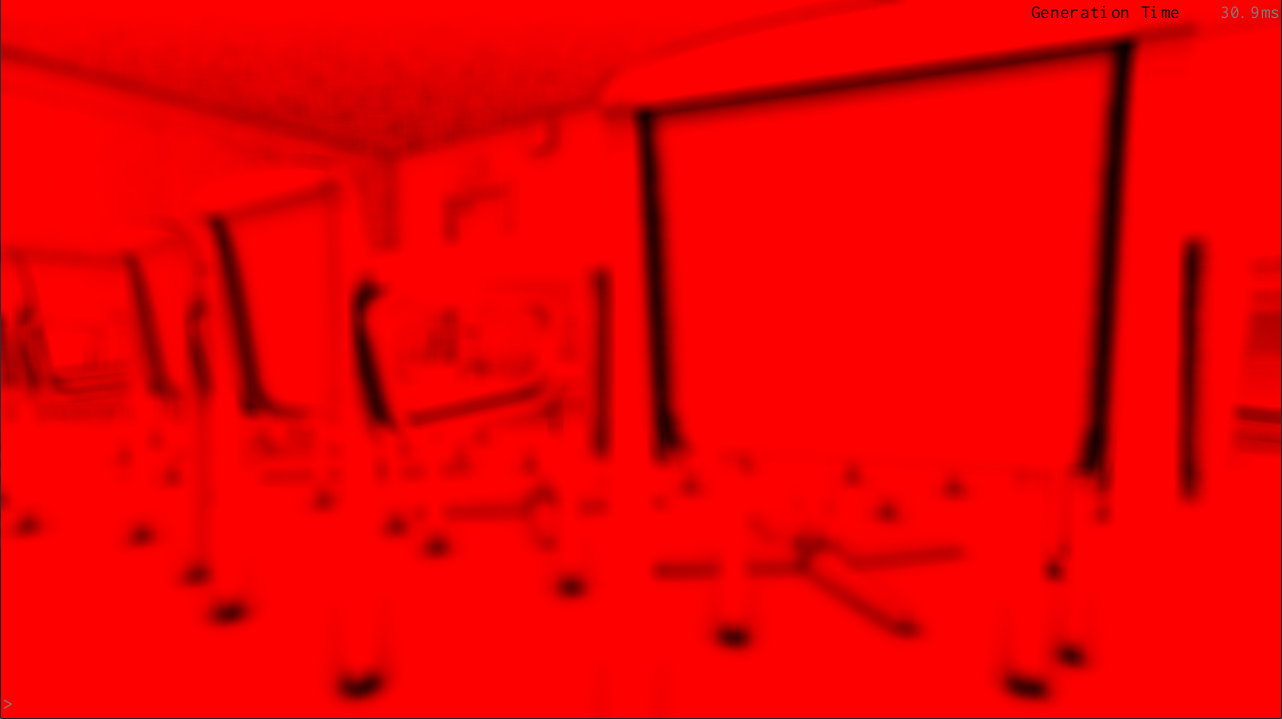
\includegraphics[scale=0.25]{img/ssao}
\end{center}
\end{frame}

%----------------------------------------------------------------------------------------

\subsection{Gaussian Filter}

\begin{frame}
\frametitle{Filtering Overview}
\begin{itemize}
\item Raw radiosity and SSAO are visibly noisy.
\begin{center}
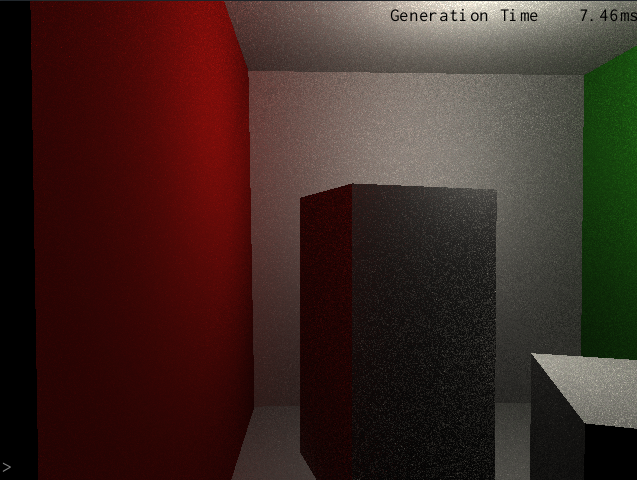
\includegraphics[scale=0.15]{img/noise}
\end{center}
\item Apply 2-pass gaussian filter:
$$B\prime_{1st}(P_{c}) = \frac{1}{W} \sum_{i = -R}^{R} \gamma(i) B(P(i,0))$$
$$B\prime(P_{c}) = \frac{1}{W} \sum_{i = -R}^{R} \gamma(i) B\prime_{1st}(P(0,i))$$
$$W = \sum_{i = -R}^{R} \gamma(i)$$
\end{itemize}
\end{frame}

\begin{frame}
\frametitle{Pure Gaussian Result}
\begin{itemize}
\item Simple Gaussian filter becomes blurry
\begin{center}
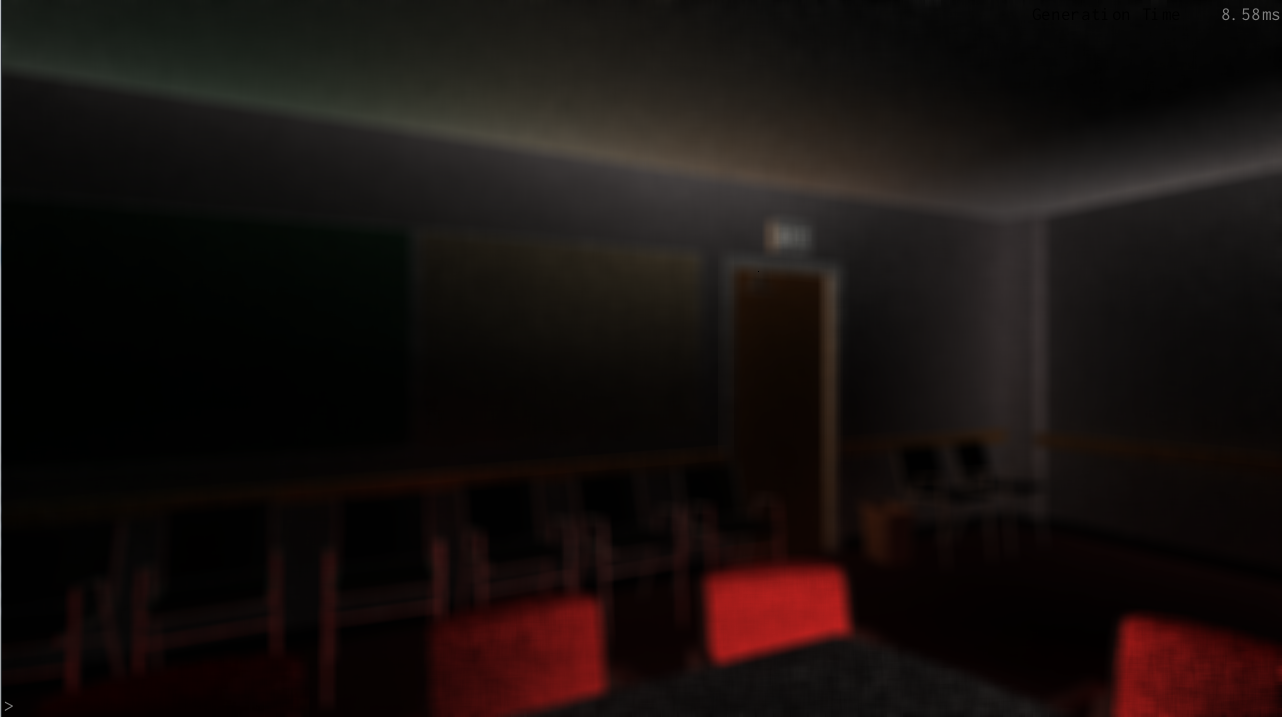
\includegraphics[scale=0.3]{img/wo-edge-rad}
\end{center}
\end{itemize}
\end{frame}

\begin{frame}
\frametitle{Edge Detection}
\begin{itemize}
\item To fix, first run edge detection algorithm:
\begin{center}
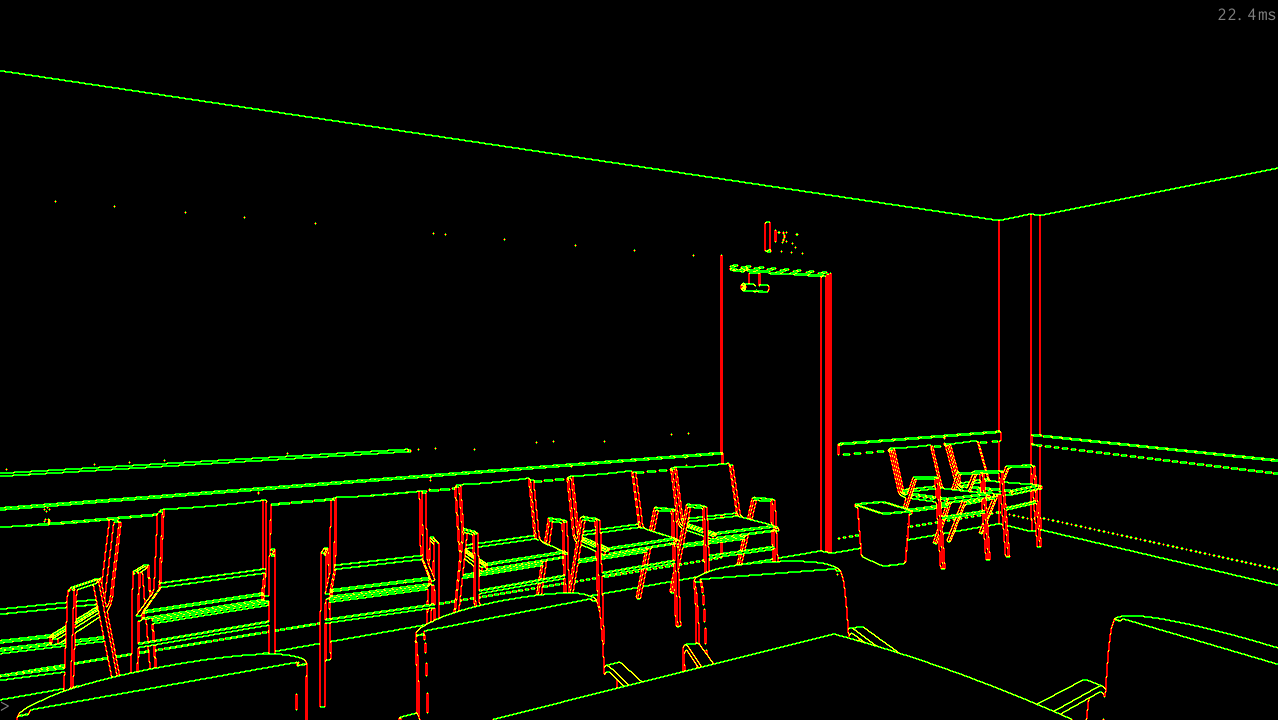
\includegraphics[scale=0.3]{img/edge-tex}
\end{center}
\end{itemize}
\end{frame}

\begin{frame}
\frametitle{Modified Filter}
\begin{itemize}
\item Stop the gaussian filter loop if it hits an edge
\begin{center}
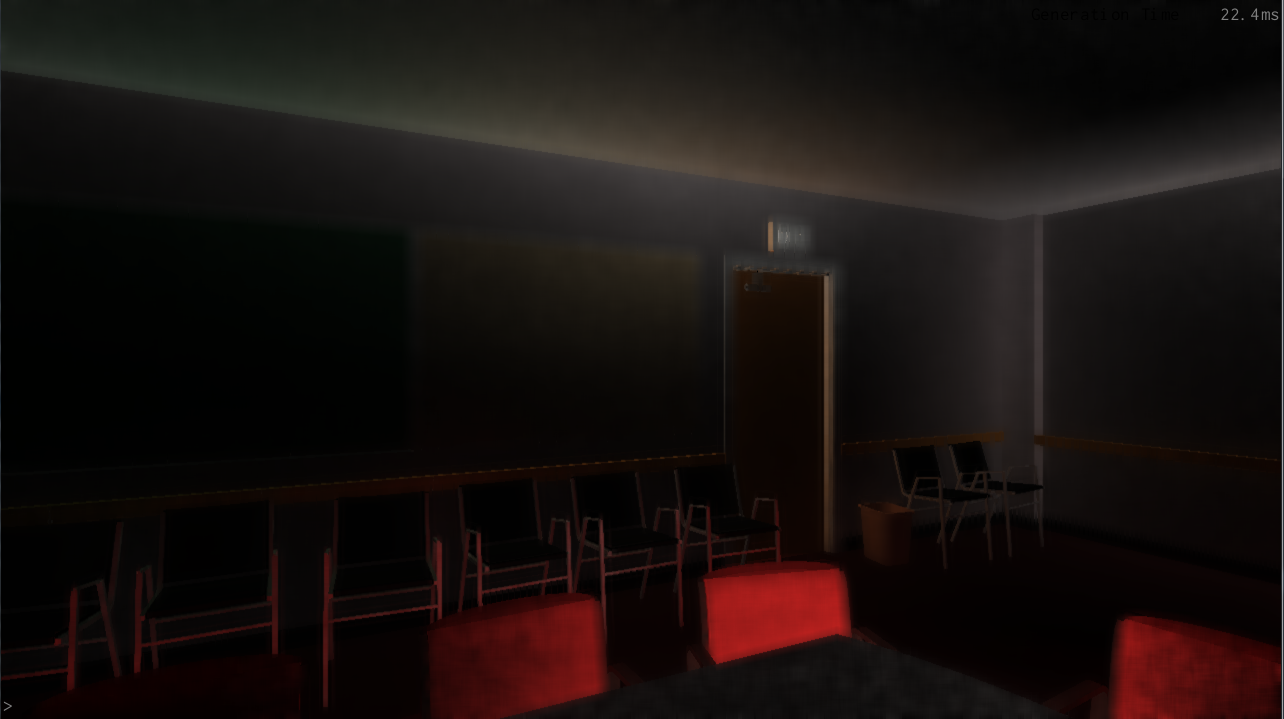
\includegraphics[scale=0.3]{img/w-edge-rad}
\end{center}
\end{itemize}
\end{frame}

\section{Conclusions}

\end{document} 